%%%%%%%%%%%%%%%%%%%%%%%%%%%%%%%%%%%%%%%%%

% Beamer Presentation
% LaTeX Template
% Version 1.0 (10/11/12)
%
% This template has been downloaded from:
% http://www.LaTeXTemplates.com
%
% License:
% CC BY-NC-SA 3.0 (http://creativecommons.org/licenses/by-nc-sa/3.0/)
%
%%%%%%%%%%%%%%%%%%%%%%%%%%%%%%%%%%%%%%%%%

%----------------------------------------------------------------------------------------
%	PACKAGES AND THEMES
%----------------------------------------------------------------------------------------

\documentclass{beamer}

\mode<presentation> {

% The Beamer class comes with a number of default slide themes
% which change the colors and layouts of slides. Below this is a list
% of all the themes, uncomment each in turn to see what they look like.

%\usetheme{default}
%\usetheme{AnnArbor}
%\usetheme{Antibes}
%\usetheme{Bergen}
%\usetheme{Berkeley}
%\usetheme{Berlin}
%\usetheme{Boadilla}
%\usetheme{CambridgeUS}
%\usetheme{Copenhagen}
%\usetheme{Darmstadt}
%\usetheme{Dresden}
%\usetheme{Frankfurt}
%\usetheme{Goettingen}
%\usetheme{Hannover}
%\usetheme{Ilmenau}
%\usetheme{JuanLesPins}
%\usetheme{Luebeck}
\usetheme{Madrid}
%\usetheme{Malmoe}
%\usetheme{Marburg}
%\usetheme{Montpellier}
%\usetheme{PaloAlto}
%\usetheme{Pittsburgh}
%\usetheme{Rochester}
%\usetheme{Singapore}
%\usetheme{Szeged}
%\usetheme{Warsaw}

% As well as themes, the Beamer class has a number of color themes
% for any slide theme. Uncomment each of these in turn to see how it
% changes the colors of your current slide theme.

%\usecolortheme{albatross}
%\usecolortheme{beaver}
%\usecolortheme{beetle}
%\usecolortheme{crane}
%\usecolortheme{dolphin}
%\usecolortheme{dove}
%\usecolortheme{fly}
%\usecolortheme{lily}
%\usecolortheme{orchid}
%\usecolortheme{rose}
%\usecolortheme{seagull}
%\usecolortheme{seahorse}
%\usecolortheme{whale}
%\usecolortheme{wolverine}

%\setbeamertemplate{footline} % To remove the footer line in all slides uncomment this line
%\setbeamertemplate{footline}[page number] % To replace the footer line in all slides with a simple slide count uncomment this line

%\setbeamertemplate{navigation symbols}{} % To remove the navigation symbols from the bottom of all slides uncomment this line
}

\usepackage{graphicx} % Allows including images
\usepackage[document]{ragged2e}
\usepackage{booktabs} % Allows the use of \toprule, \midrule and \bottomrule in tables
\usepackage[export]{adjustbox}
\usepackage{PTSansNarrow}
\usepackage[T1]{fontenc}
\usepackage{array,tabularx}
\usepackage[most]{tcolorbox}
\listoffigures
%----------------------------------------------------------------------------------------
%	TITLE PAGE
%----------------------------------------------------------------------------------------

\title[]{Multi-programming and Multitasking Operating System} % The short title appears at the bottom of every slide, the full title is only on the title page

\author[]{Arnab Bhattacharya, Tathagata Patra, Sauvik Dutta, Srikrishna Samanta} % Your name
\institute[] % Your institution as it will appear on the bottom of every slide, may be shorthand to save space
{
Department of Computer Science \\ % Your institution for the title page
\medskip
}
\date{11/10/2023} % Date, can be changed to a custom date

\begin{document}

\begin{frame}
\titlepage % Print the title page as the first slide
\end{frame}

\begin{frame}
\frametitle{Table of Contents} % Table of contents slide, comment this block out to remove it
\tableofcontents % Throughout your presentation, if you choose to use \section{} and \subsection{} commands, these will automatically be printed on this slide as an overview of your presentation
\end{frame}

%----------------------------------------------------------------------------------------
%	PRESENTATION SLIDES
%----------------------------------------------------------------------------------------

%------------------------------------------------
%\section{Overview}
%\section{Elements Of Scientific Method}
%\section{Steps of Scientific Method}
%\section{Models}
%\section{Conclusion}

% Sections can be created in order to organize your presentation into discrete blocks, all sections and subsections are automatically printed in the table of contents as an overview of the talk
%------------------------------------------------ % A subsection can be created just before a set of slides with a common theme to further break down your presentation into chunks

\section[Introduction]{Introduction}


\begin{frame}{Operating System}
    Operating System is a collection of modules which provides an efficient computing environment between hardware and software.
    
 \begin{figure}[h]
     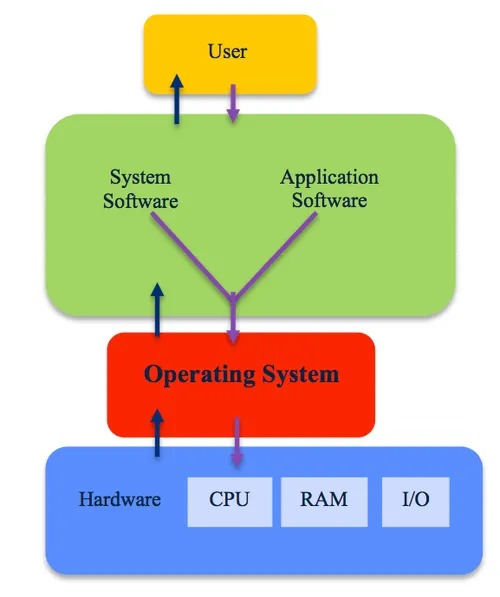
\includegraphics[width=0.35\textwidth , height=0.5\textheight]{abc}
     \caption{Role of Operating System}
     \label{fig:enter-label}
 \end{figure}
  
\end{frame}

\begin{frame}{Functions of Operating System}
\begin{itemize}
\item Process Management:
	\begin{itemize}
	\item Create, schedule, and terminate processes.
	\item Manage process communication and synchronization.
	\end{itemize}
\item Memory Management:
	\begin{itemize}
	\item Allocate and deallocate memory for processes.
	\item Implement virtual memory for efficient use of physical RAM.
	\end{itemize}
\item File Management:
	\begin{itemize}
	\item Provide access to files and directories.
	\item Handle file creation, deletion, and organization.
	\end{itemize}
\item Device Management:
	\begin{itemize}
	\item Control and interact with hardware devices.
	\item Manage device drivers and input/output operations.
	\end{itemize}
\item User Interface Interaction
	\begin{itemize}
	\item Provide a user-friendly interface (GUI/CLI).
	\item Handle user input, output, and window management.
	\end{itemize}
\end{itemize}
\end{frame}

\section{Multi-programming Operating System}

\begin{frame}{Definition of Multi-programming}
	
        \begin{itemize}
            \item Multi-programming in an operating system as the name suggests multi means more than one and programming means the execution of the program. when more than one program can execute in an operating system then this is termed a multi-programming operating system.
        \end{itemize}
        \begin{figure}[h]
        \begin{center}
        
        
        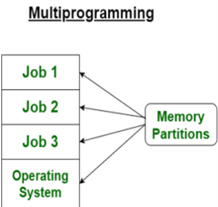
\includegraphics[width=0.45\textwidth , height=0.5\textheight]{Picture1}
        
        \end{center}
        \caption{Multiprogramming Operating System}
        \end{figure}
		
\end{frame}


\subsection{Description}
{

\begin{frame}{Operations of Multi-programming}
	
	
	\begin{minipage}{8 cm}
	\begin{itemize}
	    \item Multiple programs are to be stored in memory and each program has to be given a specific portion of memory which is known as process.
            \item Before the process undergoes execution, the operating system selects a ready process by checking which one process should undergo execution.
            \item Process need any input/output operation at that time process goes out of main memory for I/O operation and temporarily stored in secondary storage and CPU switches to next ready process.
            \item The process which undergoes for I/O operation comes again after completing the work, then CPU switches to this process.
	\end{itemize}
	
	\end{minipage}
	\hfill
	\begin{minipage}{5 cm}
	\begin{figure}
	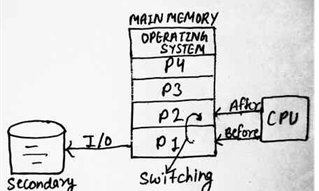
\includegraphics[width=0.8\textwidth , height=0.3\textheight]{Picture2}
	\caption{Working Principle of Multiprogramming}
	\end{figure}

	\end{minipage}
		
	\end{frame}
}

\begin{frame}{Mathematical Representation of Multiprogramming}
$c_i\in C$ Collection of CPU Cycles\\
\vskip 0.2in
$p_i\in P$ Collection of Processes\\
\vskip 0.2in
The functionality of Multiprogramming can be represented using function like this\\
f:$c_i\rightarrow\cup_{i=1}^np_i$

\end{frame}

\subsection{Pros and Cons}
{

\begin{frame}{Advantages of Multi-programming}
    \begin{itemize}
         
    
    \item  Need Single CPU for implementation.
    \item  Very high throughput.
    \item Optimal Response time.
    \item  Context Switching happens when current process undergoes waiting state.
    \item  CPU idle time is reduced.
    \item  High resource utilization.
    
    \end{itemize}
    
\end{frame}
}

\begin{frame}{Disadvantages of Multi-programming}
    \begin{itemize}
        \item If it has a large number of jobs, then long-term jobs will have to require a long wait.
        \item Memory management is needed in the operating system because all types of tasks are stored in the main memory.
    \end{itemize}
    
\end{frame}

\section{Multitasking Operating System}

\subsection{Description}

\begin{frame}{Definition of Multitasking}
	\begin{minipage}{5 cm}
	
	    
    \begin{itemize}
        \item Multi tasking operating systems allow multiple users to perform multiple tasks at the same time. The allocation of system resources such as input/output devices, CPU and memory among processes can be easily managed by multi-tasking operating system.
        \item Multitasking is the ability of an OS to execute more than one task simultaneously on a CPU machine.
    \end{itemize}
    \end{minipage}
    \hfill
    \begin{minipage}{8 cm}
    \begin{figure}
    
    
    	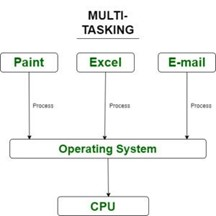
\includegraphics[width = 0.5\textwidth, height = 0.5\textheight]{Picture3}
    	\caption{Multitasking Operating System}
    	\end{figure}
    \end{minipage}
\end{frame}

\begin{frame}{Mathematical Representation of Multitasking}

$c_i\in P$ Collection of CPU Cycle\\
\vskip 0.2in
$T_i\in T$ Collection of User tasks\\
\vskip 0.2in
m is no. of CPU cores
\vskip 0.2in
n is no. of processes in each core
\vskip 0.2in
The functionality of Multitasking can be represented using function like this\\
f:${c_i}^m\rightarrow\cup_{i=1}^nT_i$

\end{frame}

\begin{frame}{Features of Multitasking}
    \begin{minipage}{7 cm}
    \begin{itemize}
        \item Time Sharing – In this, many processes are allocated with resources of computer in respective time slots, processors time is shared with multiple processes.
        \item Context Switching – Context switching is a process of saving the context of one process and loading the context of another process.
        \item Hardware Interrupt – When a process or an event requires urgent attention, hardware or software will signal with an interrupt. It informs the processor that a high-priority task has arisen that necessitates interrupting the running process.
    \end{itemize}
    
    \end{minipage}
    \hfill
    \begin{minipage}{5 cm}
    \begin{figure}
    
    
    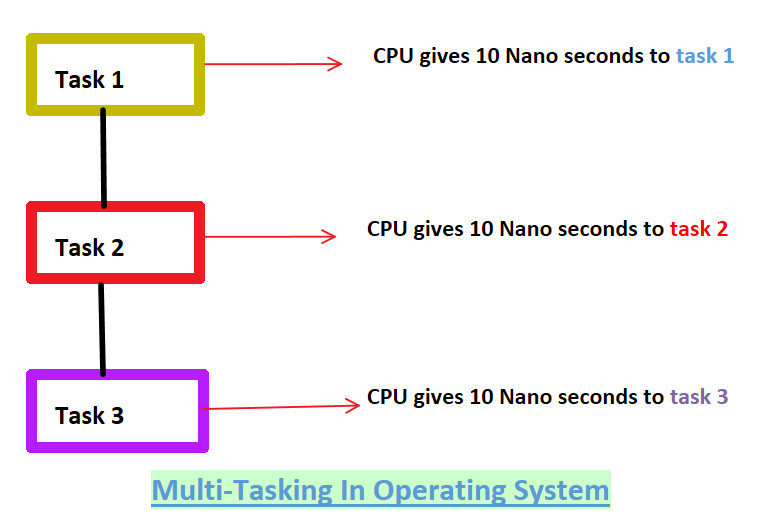
\includegraphics[width = 1.0\textwidth, height = 0.4\textheight]{Multitasking-in-operating-system}
    \caption{Working Principle of Multitasking}
\end{figure}    
    \end{minipage}
\end{frame}



\subsection{Pros and Cons}

\begin{frame}{Advantages of Multitasking}
    \begin{itemize}
        \item Multi-Tasking Operating System is capable of executing multiple application simultaneously without slowing down the system.
        \item Each process is assigned specific length of time(i.e time sharing), hence a process does not have to wait for longer duration to utilize CPU. Starvation of process is not found in these operating system.
        \item A multitasking OS can effectively manage I/O devices, RAM, hard disks, CPU, and other computer resources.
    \end{itemize}
\end{frame}

\begin{frame}{Disadvantages of Multitasking}
    \begin{itemize}
        \item As a single processor is executing multiple processes at the same time then there will be load on CPU.
        \item Computer system will be lagging if the processor is slow in Multi-Tasking Operating System while executing multiple programs simultaneously.
    \end{itemize}
\end{frame}



\section{Comparison between Multiprogramming and Multitasking}



\begin{frame}{Comparison between Multiprogramming and Multitasking}
	
	
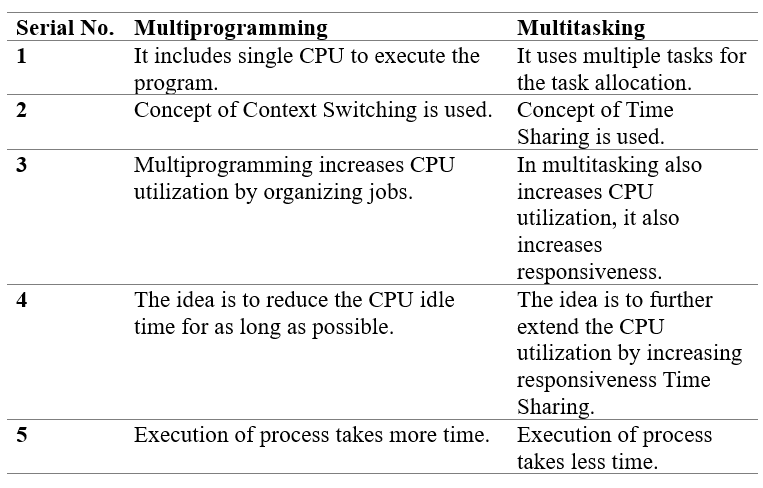
\includegraphics[width=1\textwidth, height=0.85\textheight]{ss1}

\end{frame}

%------------------------------------------------


%------------------------------------------------

\begin{frame}
\Huge{\centerline{Thank You}}
\end{frame}

%----------------------------------------------------------------------------------------

\end{document}